\section{Reading Note: Comets, Gantert and Zeitouni, RWRE large deviation principle}

\subsection{Main results, qualitative discussion}


\subsection{Outline of proof}

\subsection{Quenched LDP for hitting times}


\begin{lem}[Lemma 1]
	\label{lem:Comet00Lemma1}
	For any $\lambda \in \mathbb{R}$, we have that whenever $\varphi(\lambda, \omega)<\infty$ a.s. then

\[
\varphi(\lambda, \omega)=\frac{1 \mid}{\mid e^{-\lambda}\left(1+\rho_0(\omega)\right)}-\frac{\rho_0(\omega) \mid}{\mid e^{-\lambda}\left(1+\rho_{-1}(\omega)\right)}-\frac{\rho_{-1}(\omega) \mid}{\mid \cdots}
\]


Further, for $\eta \in M_1^e(\Sigma)^{+, K}$ and $1<u<E_\eta\left[\tau_1\right]:=\int E_\omega\left[\tau_1\right] \eta(d \omega) \leq \infty$, there exists a unique $\lambda_0=\lambda_0(u, \eta)$ such that $\lambda_0<0$ and

\[
u=\left.\int \frac{d}{d \lambda} \log \varphi(\lambda, \omega)\right|_{\lambda=\lambda_0} \eta(d \omega)
\]


Finally, for u as above

\[
\inf _{\eta \in M_1^e(\Sigma)^{+}, K} \lambda_0(u, \eta)>-\infty
\]
\end{lem}

To understand this proof, first recall the Quenched LDP:
\[
	I_ \eta ^{\tau, q} (u) = \sup _\lambda \lambda u - \mathbb{E}\left[ \log E_\omega \left[ e^{\lambda \tau_1} 1_{\tau_1< \infty } \right]  \right] 
.\] 
Write $\varphi(\lambda, \omega) = E_\omega\left[ e^{\lambda \tau_1} 1_{\tau_1 < \infty } \right] $. In this theorem, we work with $\eta \in M_1^e(\Sigma)^{+, K}$, so $\varphi(\lambda, \omega) = E_\omega\left[ e^{\lambda \tau_1}\right] $. This reduction is crucial for the arguments in this Lemma. We will deal with general, i.e. nestling case later using a reflection argument.

We first recall the fact from LDP:

\begin{tcolorbox}[title=,colback=gray!10,colframe=black,breakable]
	Let $f: \mathbb{R} \to  \mathbb{R}$ be a convex $C^1$ function where $f'$ takes all values in $(a,b)$. Then for every $u \in (a,b)$, the Legendre transform of $f$, $I(u) = \sup _\lambda \lambda u - f$ is exactly defined by $I(u) = \lambda_0 u - f(\lambda)$ where $\lambda_0 \in \mathbb{R}$, $f'(\lambda_0) = u$. Moreover, $\lambda_0 (u)$ is monotone. If $f$ is strictly convex, $\lambda_0(u)$ is continuous.
\end{tcolorbox}

Write $f(\lambda) = \mathbb{E}\left[ \log \varphi(\lambda, \omega) \right] $
Let's compute:
\begin{align*}
	\frac{d }{d \lambda} f 
	&= \int \frac{d }{d \lambda} \log E_\omega \left[ e^{\lambda \tau_1} \right] \eta(d \omega) \\
	&= \int \frac{E_\omega \left[ \tau_1 e^{\lambda \tau_1} \right]}{E_\omega \left[ e^{\lambda \tau_1} \right]}  \eta(d \omega)
.\end{align*}
Now, analyze the behavior of integrand w.r.t. $\lambda$, recall that \strategy{Laplace's Principle identifies extremum of a nice function}, we have
\begin{itemize}
	\item When $\lambda \to \infty $, $\frac{E_\omega \left[ \tau_1 e^{\lambda \tau_1} \right]}{E_\omega \left[ e^{\lambda \tau_1} \right]} \to \operatorname{esssup } \tau_1 = \infty $.
	\item When $\lambda \to -\infty $, $\frac{E_\omega \left[ \tau_1 e^{\lambda \tau_1} \right]}{E_\omega \left[ e^{\lambda \tau_1} \right]} \to \operatorname{essinf } \tau_1 = 1 $.
	\item When $\lambda = 0$, $\frac{d }{d \lambda} f = \mathbb{E}\tau_1$.
\end{itemize}

Thus, for $1<u<E_\eta\left[\tau_1\right]$, we have  $\lambda_0 \in (- \infty , 0)$. This proves the second claim.

To prove the third claim, we first note that $u_\lambda := \frac{d }{d \lambda} f \to 1$ as $\lambda \to -\infty $ uniformly in $\eta$. To see this, compute the bound


\begin{align*}
	1 \le \frac{E_\omega \left[ \tau_1 e^{\lambda \tau_1} \right] }{E_\omega \left[ e^{\lambda \tau_1} \right] } 
	&= \frac{\omega_0 e^\lambda + E_\omega \left[ \tau_1 e^{\lambda \tau_1} \mathbf{1}_{\tau_1 \ge 2} \right] }{\omega_0 e^\lambda} \\
	&\leq 1 + \frac{c e^{\lambda / 3}}{ \omega_0}
.\end{align*}

The second inequality is due to
\[
	E_\omega \left[ \tau_1 e^{\lambda \tau_1} \mathbf{1}_{\tau_1 \ge 2} \right]
	= E_\omega \left[ \tau_1 e^{\lambda \tau_1 / 3}e^{2 \lambda \tau_1 / 3} \mathbf{1}_{\tau_1 \ge 2} \right]
	\le \frac{3}{\lambda e} e^{4 \lambda / 3}
.\] 

Using uniform ellipticity, the right hand side converges to $1$ uniform in $\omega$. Hence the expectation over $\mathbb{E}_\eta$ converges uniformly in $\eta$.

Now, this means for all $\varepsilon>0$ there exists $M > 0$ such that for all  $\eta$, $\lambda$, we have 
\[
	\lambda < - M \implies u_\lambda^{(\eta)} < 1 + \varepsilon
.\] 
By previous observation we see that $\lambda \mapsto u_\lambda$ is invertible, i.e. $\lambda_0(u_\lambda) = \lambda$. Thus for all $u$,
\[
	\lambda_0(u, \eta) < - M \implies u < 1 + \varepsilon
.\] 

But $u$ is fixed, so $\lambda_0(u, \eta) > - M$ uniformly in $\eta$.

The first statement, continued fraction representation, is proved using pathwise decomposition on the first step. From the proof and the formula we see that influence of $\omega$ on $\varphi$ decreases exponentially the further away from the origin.

\begin{lem}[Lemma 2]
	\label{lem:Comet00Lem2}
	Lemma 2. Let $\eta \in M_1^e(\Sigma)^{+, K}$. Then
(i) There is a deterministic $\infty>\lambda_{\text {crit }} \geq 0$, depending only on $\eta$, such that for $\lambda<\lambda_{\text {crit }} \varphi(\lambda, \omega)<\infty$ for $\eta$-a.e. $\omega$, and for $\lambda>\lambda_{\text {crit }} \varphi(\lambda, \omega)=\infty$ for $\eta$-a.e. $\omega$.
(ii) Let $u_{\text {crit }}=\infty$ if $\int E_\omega\left[\tau_1 e^{\lambda_{\text {crit }} \tau_1}\right] \eta(d \omega)=\infty$ and $u_{\text {crit }}:=\left.\int \frac{d}{d \lambda} \log \varphi(\lambda, \omega)\right|_{\lambda=\lambda_{\text {crit }}} \eta(d \omega)$ otherwise. For $E\left[\tau_1\right] \leq u<u_{\text {crit }}$, there exists a unique $\lambda_0=\lambda_0(u, \eta)$ such that $\lambda_0 \geq 0$ and (15) holds.
\end{lem}
\begin{proof}
	To prove (1): Define $\lambda_c(\omega) = \sup \{\lambda : E_\omega \left[ e^{\lambda \tau_1} \right] < \infty \} $. However, finiteness of this quantity should not be affected by translations, so $\lambda_c(\omega) = \lambda_c (\theta \omega)$. Apply the Ergodic Theorem, we have $\mathbb{E}_ \eta \left[ \lambda_c(\omega) \right] = \lambda_c(\omega)$, i.e. $\lambda_c(\omega)$ is deterministic and only depends on $\eta$.

	To prove (2): This is entailed by our analysis in the last lemma.
\end{proof}

Combining the two lemmas, we are able to prove the quenched LDP of hitting times in the right transient or recurrent case.

\begin{thm}[Theorem 4]
	\label{thm:Comet00Thm4}
Assume $\eta \in M_1^e(\Sigma)^K$. Then, for $\eta$-a.e. $\omega$, the distributions of $T_n / n$ under $P_\omega$ satisfy a weak LDP with deterministic, convex rate function $I_\eta^{\tau, q}$. Further, $I_\eta^{\tau, q}(\cdot)$ is decreasing on $\left[1, \int \tau_\omega \eta(d \omega)\right]$ and increasing on $\left[\int \tau_\omega \eta(d \omega), \infty\right)$.	
\end{thm}
\begin{proof}[Proof in the $\eta \in M_1^e(\Sigma)^{K, +}$ case]

	\textbf{Upper bound.} We want to show, for $1 < u \le \mathbb{E}_ \eta [\tau_1]$ and $\eta \in M_1^e (\Sigma)^{+, K}$ (recurrent or right transient), the identity
	\[
		\limsup_{n \to \infty} \frac{1}{n} \log P_\omega \left[ \frac{1}{n} \sum_{j=1}^{n} \tau_j \le u \right] \le - \sup _{\lambda \in \mathbb{R}} \lambda u - \mathbb{E}_ \eta \left[ \log \varphi (\lambda, \omega) \right] \triangleq - I_\eta ^{\tau, q}(u)
	,\]
	and for $\mathbb{E}_ \eta [\tau_1] \le  u < \infty $,
	\[
		\limsup_{n \to \infty} \frac{1}{n} \log P_\omega \left[ \frac{1}{n} \sum_{j=1}^{n} \tau_j \ge u \right] \le - \sup _{\lambda \in \mathbb{R}} \lambda u - \mathbb{E}_ \eta \left[ \log \varphi (\lambda, \omega) \right] \triangleq - I_\eta ^{\tau, q}(u)
	.\]
	
	We treat the first case and simply note that the second case has a symmetrical proof. 

	Note the general shape of $\mathbb{E}\log \varphi(\lambda, \omega)$, we see that $1 < u \le \mathbb{E}_ \eta [\tau_1]$ corresponds with $\lambda \le 0$. Recall the \strategy{exponential change of measure} in Cramer's theorem, we have
	\begin{align*}
		P_\omega \left[ \frac{1}{n} \sum_{j=1}^{n} \tau_j \le u \right]
		&= P_\omega \left[ e^{\lambda\sum_{j=1}^{n} \tau_j } \ge e^{\lambda n u} \right] \\
		&\leq E_\omega \left[ e^{\lambda\sum_{j=1}^{n} \tau_j } \right] e^{- \lambda n u} \\
	.\end{align*}
	Using \strategy{independence of hitting times} and the \strategy{ergodic theorem} we have
	\[
		\frac{1}{n} \log  P_\omega \left[ \frac{1}{n} \sum_{j=1}^{n} \tau_j \le u \right]
		\le - \left(\lambda u - \frac{1}{n} \sum_{j=1}^{n}\log \varphi(\lambda, \theta^j \omega)\right) 
		\to - \left( \lambda u - \mathbb{E}_ \eta \log \varphi(\lambda, \omega) \right) 
	.\] 
	A tiny technical point: the ergodic theorem says this convergence happens $\eta$-a.s. for each $\lambda$. This implies $\eta$-a.s. this holds for all $\lambda \in \mathbb{Q}$. Using the monotonicity and continuity of both sides w.r.t. $\lambda$, we conclude that $\eta$-a.s. the convergence holds for all $\lambda \in \mathbb{R}$. 

	By Lemma~\ref{lem:Comet00Lemma1}, the supremum is attained at $\lambda_0(u)$ and further is equal to supremum over $\lambda \in \mathbb{R}$. Therefore
	\[
		\limsup_{n \to \infty} \frac{1}{n} \log P_\omega \left[ \frac{1}{n} \sum_{j=1}^{n} \tau_j \le u \right] \le  - I_\eta ^{\tau, q}(u)
	.\] 

	For the second case, use the same proof. The only difference is that $\lambda_0(u_{\text{crit}}) = \lambda_{\text{crit}}$.

	\textbf{Lower Bound.} This is the harder part. This is harder because $\tau_j$ may not have all moments (i.e. $\lambda_{\text{crit}}< \infty $ in Lemma~\ref{lem:Comet00Lem2}). To deal with this, we restrict ourselves to events $A_{n, M} = \{\tau_j \le M, j = 1, \ldots, n\} $ and derive the LDP on these restricted events. Since $P_\omega \left[ \tau_1 < M \right] \uparrow P_\omega \left[ \tau_1 < \infty  \right]  = 1$ (our assumption on $\eta$ is crucial here), in the scale $\frac{1}{n} \log \left( \cdot  \right) $ the effect of such change of measure vanishes as $M \to \infty $.

	We make the following definitions:
	\begin{align*}
		\varphi_M(\lambda, \omega) &= E_\omega \left[ \mathbf{1}_{\tau_1 \le M} \right] \\
		\tilde \varphi _M(\lambda, \omega) &= \tilde E _\omega \left[ e^{\lambda \tau_1} \right]  = \varphi_M(\lambda, \omega) / P_\omega \left[ \tau_1 \le  M \right] 
	.\end{align*}
	We have
	\[
		\mathbb{E}_\eta \log \tilde \varphi_M(\lambda, \omega)
		= \mathbb{E}_\eta \log \varphi_M(\lambda, \omega) - C_M, \qquad C_M \to_{M \to \infty } 0
	.\] 

	Thus 
	\[
		\frac{1}{n} \log P_\omega\left[ \frac{1}{n} \sum_{j=1}^{n} \tau_j \in  (u - \delta, u + \delta) \right] 
		\ge 
		\frac{1}{n} \log \tilde P_\omega\left[ \frac{1}{n} \sum_{j=1}^{n} \tau_j \in  (u - \delta, u + \delta) \right] 
		+ \frac{1}{n} \log P_\omega(A_{n, M})
	,\] 
	where the second term ?picis insignificant. Now, lets looks at $\tilde \varphi_M$, the MGF under the changed measure. 
	
	\begin{figure}[H]
		\centering
		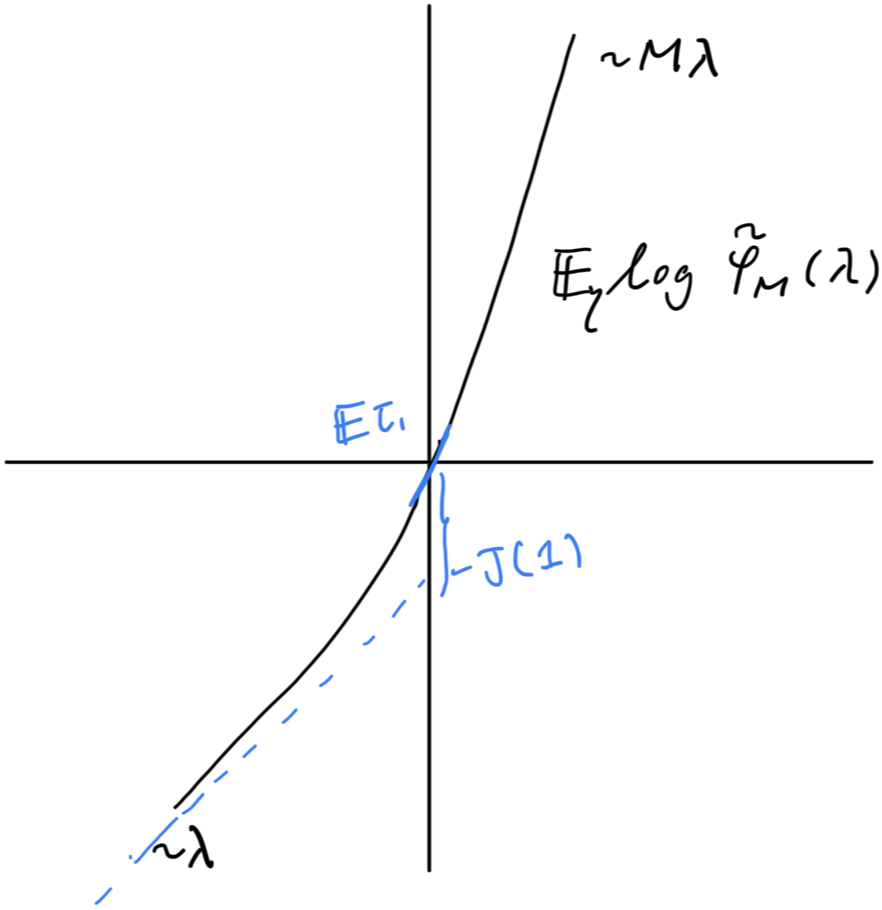
\includegraphics[width=0.5\textwidth]{src/Comet00-mgf-tildeM.png}
		\caption{The function $\tilde \varphi_M(\lambda)$}
		\label{fig:Comet00-1}
	\end{figure}

	We see that this is a smooth and convex function, so by property of Lagendre transform (similar to proof of Theorem 1), for each  $u \in (1, \infty )$ and $M > u$ we may choose $\lambda_M(u)$ such that
	\[
		 u = \int \frac{d}{d \lambda} \log \tilde \varphi_M(\lambda, \omega) |_{\lambda = \lambda_M(u)} \eta (d \omega)
	.\] 

	Now we can apply \strategy{exponential change of measure}:
	\begin{align*}
		&E^{\tilde P_{\omega, M, \lambda_M(u)}}  \left[ 
			\mathbf{1}_{\frac{1}{n} \tau_i \in (u - \delta, u + \delta)}
		\frac{e^{\lambda_M(u) \sum \tau_i}}{\tilde E_\omega e^{\lambda_M(u) \sum \tau_i}} 
		\frac{\tilde E_\omega e^{\lambda_M(u) \sum \tau_i}}{e^{\lambda_M(u) \sum \tau_i}}
	\right] \\
	&= E^{\tilde Q_{\omega, M, \lambda_M(u)}} 
	\left[ \mathbf{1}_{\frac{1}{n} \tau_i \in (u - \delta, u + \delta)} e^{-\lambda_M(u) \sum \tau_i} \right] \tilde E_\omega e^{\lambda_M(u) \sum \tau_i} \tilde Q \left[ \left| \frac{1}{n} \sum \tau_i - u \right| < \delta \right] \\
	&\ge \exp \left( - n \lambda_M(u) (u \pm \delta) + \sum_j \log \tilde \varphi_M(\lambda_M(u), \theta^j \omega) \right) 
	\tilde Q \left[ \left| \frac{1}{n} \sum \tau_i - u \right| < \delta \right] 
	.\end{align*}

	From here, note three things:
	\begin{enumerate}
		\item Under the changed measure $Q = Q_{\omega, M, \lambda_M(u)}$, we have
			\[
				\mathbb{E}_ \eta E^{\tilde Q} \tau_1 = \mathbb{E}_ \eta E^{\tilde P_M} \frac{\tau_1 e^{\lambda \tau_1}}{E^{\tilde P_M} e^{\lambda \tau_1}} = \mathbb{E}_ \eta \frac{d }{d \lambda} \log \tilde \varphi (\lambda, \omega) = u
			.\] 
		\item Under $Q$, we have the SLLN-like result since the $\tau_j$ remain independent: (c.f. Durett Thm 2.3.5)
			\[
				E^{\tilde Q_\omega}  \left[ \frac{1}{n} \sum_{j=1}^{n} \left(\tau_j - E^{\tilde Q_\omega}\tau_j \right)^4 \right]  \le 3 M^4 / n^2
			.\] 
		Then using Borel-Cantelli, for $\eta$-a.e. $\omega$, 
		\[
			\tilde Q \left[ \left| \frac{1}{n} \sum_{j = 1}^n \tau_j - E^{\tilde Q_\omega} \tau_j \right| < \delta \right]
		.\] 
		\item The ergodic theorem tells us that
			\[
				\frac{1}{n} \sum_{j = 1}^n E^{\tilde Q_\omega} \left[ \tau_j \right] \to \mathbb{E}_ \eta E^{\tilde Q_\omega} \tau_1 = u
	\] 
	as $n \to \infty $, for all $u, M$, for $\eta$-a.e. $\omega$.
	\end{enumerate}
	From the above, we conclude that
	\[
		\tilde Q \left[ \left| \frac{1}{n} \sum \tau_i - u \right| < \delta \right] \to 1
	.\] 

	Now, taking logarithm, dividing by $n$ and taking $n \to \infty $, and then $\delta \to 0$, we have $\eta$-a.s.,
	\begin{align*}
		&\lim_{\delta \to 0} \liminf_{n \to \infty } \frac{1}{n} \log \tilde P_\omega \left[ \frac{1}{n} \sum_{j=1}^{n} \tau_j \in  (u - \delta, u + \delta) \right] \\
		& \ge -\left(\lambda_M(u) u-\liminf _{n \rightarrow \infty} \frac{1}{n} \sum_{j=1}^n \log \tilde{\varphi}_M\left(\lambda_M(u), \theta^j \omega\right)\right) \\
		&= - \left( \lambda_M(u) u - \mathbb{E}_ \eta \log_M(\lambda_M(u), \omega)\right)  - C_M \\
		&\ge  - \sup _{\lambda \in \mathbb{R}} (\lambda u -\log \varphi_M(\lambda)) - C_M := - I_M(u) - C_M
	.\end{align*}

	Let's try to understanding $I_M(u)$. As $M \to \infty $, we expect  $\varphi_M \uparrow \varphi$, and hence $I_M \downarrow I_\eta ^{\tau, q}$. (Picture here.) Therefore, we define
	\[
		I^*(u) = \limsup _{M \to \infty } I_M(u)
	.\] 
	Thus, $I^*(u) \ge 0$ and $I^*(u) < \infty $. We see that the sets $\{\lambda: \lambda u - \log \varphi_M(\lambda) \ge I^*(u)\} $ are nonempty ($\lambda_M(u)$ ), compact (for $M > u$), and nested. Hence contain some $\lambda^* < \infty $ in their intersection. By Lebesgue's monotone convergence, we get
	\[
		\mathbb{E}_ \eta \log \varphi_M(\lambda^*, \omega) \to \mathbb{E}_ \eta \log \varphi(\lambda^*, \omega) \le  \lambda^* u - I^*(u)
	.\] 
	From this, we have
	\begin{align*}
		& \liminf_{M \to \infty } - I_M(u) - C_M\\
		&\geq - \limsup I_M(u) \\
		&\triangleq - I^*(u) \\
		&\geq - \left( \lambda^* u - \mathbb{E}_ \eta \log \varphi(\lambda^*, \omega)\right) \\
		&\geq - \sup _{\lambda \in \mathbb{R}}\left( \lambda u - \mathbb{E}_ \eta \log \varphi(\lambda, \omega)\right) \\
		&\triangleq - I_ \eta^{\tau, q}(u)
	.\end{align*}

\end{proof}


\begin{proof}[Proof for $\eta \in M_1^e(\Sigma)^{-, K}$ ]
	\textbf{Intuition.} In the left-transient or recurrent case, the LDP for $T_n / n$ describes the speed of \textit{backtracking}, and are composed with two parts: 1) The probability of hitting $1, \ldots, n$ before going to $\to \infty $;  2) The probability of achieving some speed given that hitting occurs.

	\textbf{Step 1: Condition on Hitting.} Define $\overline{\tau} _{-1}, \overline{\tau} _{-2}, \ldots, \overline{\tau} _{-N}$ to have same distribution with $\tau_{-1}, \tau_{-2}, \ldots, \tau_{-N}$, conditioned on $T_{-N } < \infty $. That is, if we write $P_{\overline{\omega} , N} := P_\omega \left[ \cdot  | T_{-N} < \infty  \right] $, then $P_{\overline{\omega} , N}(A_{\tau_{-1}, \ldots, \tau_{-N}}) = P_\omega (A_{\overline{\tau} _{-1}, \ldots, \overline{\tau} _{-N}}) $. We see that
	\begin{itemize}
		\item $\overline{\tau} _{-1}, \ldots, \overline{\tau} _{-N}$ are independent under $P_\omega$ and form a stationary sequence under $P$.
		\item $\overline{\tau} _{-j}$ does not depend on $N$, and the extension of $\left( P_{\overline{\omega} , N} \right) _{N \ge 1}$ is the distribution of the Markov chain with transition probabilities $\overline{\omega} _i = \omega_i P_{\theta^{i + 1}\omega}(T_{-1} < \infty )$.
	\end{itemize}
	To see this,
	\begin{align*}
		P_{\overline{\omega} , N} \left( X_{n + 1} = x_n + 1 | X_1^n = x_1^n \right) 
		&= \frac{P_\omega \left( X_{n + 1} = x _{n} + 1 , x_1^n = x_1^n, T_{-N} < \infty  \right) }{P_\omega\left( X_1^n = x_1^n, T_{-N} < \infty  \right) } \\
		&= \frac{P_\omega\left( X_{n + 1} = x_{n} + 1, X_1^n = x_1^n \right)}{P_\omega\left( X_1^n = x_1^n \right) } 
		{\color{blue} \frac{P_\omega \left( T_{-N} < \infty  | x_1^{n + 1} \right) }{P_\omega \left( T_{-N }< \infty  | x_1^n \right) } }\\
		&= \omega_{x_n} P_\omega^{x_{n} + 1} \left( \tau_{x_n} < \infty  \right) = \omega_{x_n} P_{\theta^{x_n + 1} \omega}\left( \tau_{-1} < \infty  \right) 
	.\end{align*}
	To explain the blue part: if the walk reaches from $x_n + 1$ to $x_n$ in finite time, and reaches from $x_n$ to $-N$ in finite time, then $T_{-N} < \infty $.	

	Having established those properties, we define
	\begin{align*}
		\overline{\varphi} (\lambda, \omega) &= E_\omega e^{\lambda \overline{\tau} _{-1}} = \tilde \varphi(\lambda, \omega) / P(\tau_{-1} < \infty )\\
		\tilde \varphi (\lambda, \omega) &= E_\omega e^{\lambda \tau_{-1}} 1_{\tau_{-1} < \infty }
	.\end{align*}

	\textbf{Step 2: Backtracking LDP conditioned on hitting.}
	Now it is natural to consider the following LDP:
	\begin{thm}[Theorem 6]
		$\left( \frac{1}{n} \sum_{j = 1}^n \overline{\tau} _{- j} \right) _n$ satisfies L.D.P. with rate $n$, and rate function $I_ \eta ^{\tau, q}$.
	\end{thm}
	We expect the rate function to be identical to the $\tau_j$ case, in the $\eta \in M_1^e(\Sigma)^{+, K}$ case.
	The proof will be identical to that case, so the theorem follows from
	\begin{lem}
		For all $\eta \in M_1^e(\Sigma)^{+, K}$ and $\lambda \in \mathbb{R}$,
		\[
			\int \log \overline{\varphi}(\lambda, \omega)  \eta(d \omega)
			= \int \log \varphi(\lambda, \omega) \eta(d \omega)
		.\] 
	\end{lem}

	This is equivalent to
	\[
		\int \log \tilde \varphi \eta(d \omega)
		= \int \log \varphi \eta(d \omega)
		+ \int  \log P(\tau_{-1} < \infty ) \eta(d \omega)
	.\] 
	To evaluate $P(\tau_{-1} < \infty )$ term, recall
	 \[
		P_\omega \left[ \min_k X_k \le - n \right] 
		= \frac{R(0, \infty )}{ R(0, -n) + R(0, \infty )}
	.\] 
	Thus
	\begin{align*}
		P_\omega(\tau_{-1} < \infty )
		&= \frac{R(0,\infty )}{R(0,\infty ) + R(-1, 0)}\\
		&= \frac{\sum_{k=0}^{\infty} \rho_k \ldots\rho_0 }{1 + \sum_{k=0}^{\infty} \rho_k \ldots\rho_0}\\
		&= \rho_0\frac{1 + \sum_{k=1}^{\infty} \rho_k \ldots\rho_0 }{1 + \sum_{k=0}^{\infty} \rho_k \ldots\rho_0}
	.\end{align*}
	The ergodic theorem implies
	\[
		E \log P_\omega(\tau_{-1} < \infty ) = E \log \rho_0
	.\] 

	Thus, we want to show
	\[
		\left\langle \log \tilde \varphi \right\rangle 
		= \left\langle \log \varphi \right\rangle  + \left\langle \log \rho_0 \right\rangle 
	.\] 
	Let $\lambda$ be such that $\left\langle \log \varphi \right\rangle  < \infty $. Consider $D_M = \{\tau_{-1} < T_M\} $, $\tilde \varphi_M (\lambda, \omega) = E_\omega \left[ e^{\lambda \tau_{-1}}; D_M \right] $. Then, on $D_M$, $T_M = \tau_{-1} + \tau_{1}' + T_M'$ are all independent. Apply path decomposition, we obtain, as $E_\omega e^{\lambda T_M} < \infty $,
	\[
		E_\omega\left[ e^{\lambda T_M; D_M} \right] 
		= \tilde \varphi^M (\lambda, \omega) \varphi(\lambda, \theta^{-1} \omega) E_\omega \left[ e^{\lambda T_M} \right] 
	.\] 
	Hence
	\[
		1 \ge \frac{E_\omega\left[ e^{\lambda T_M; D_M} \right]}{E_\omega\left[ e^{\lambda T_M} \right]} = \tilde \varphi^M(\lambda, \omega) \varphi(\lambda, \theta^{-1} \omega)
	.\] 
	Hence
	\[
		- \log \varphi(\lambda, \theta^{-1} \omega) \ge  \log \tilde \varphi(\lambda, \omega) \ge \log \tilde \varphi^M(\lambda, \omega) \uparrow \log \tilde \varphi(\lambda, \omega)
	.\] 
	Hence
	\[
		- \log \varphi(\lambda, \theta^{-1} \omega) 
		\ge \log \tilde \varphi(\lambda, \omega) 
		\ge \log \tilde \varphi^M(\lambda, \omega)
		\ge \lambda + \log(1 - \omega_0)
	.\] 
	Therefore $\tilde \varphi^M$ is integrable. Now, we want to relate $\varphi$ and $\tilde \varphi^M$. We have two pathwise decomposition equations:
	\[
		\begin{cases}
			\tilde\varphi(\lambda, \omega) 
			= (1 - \omega_0)e^\lambda + \omega_0 e^\lambda \tilde \varphi^{M - 1}(\lambda, \theta \omega) \tilde \varphi^M(\lambda, \omega) \\
			\varphi(\lambda, \omega) = \omega_0 e^\lambda + (1 - \omega_0) e^\lambda \varphi(\lambda, \theta^{-1} \omega) \varphi(\lambda, \omega)
		\end{cases}
	.\] 
	To foster intuition, we represent them as the following digram:

	\begin{figure}[H]
		\centering
		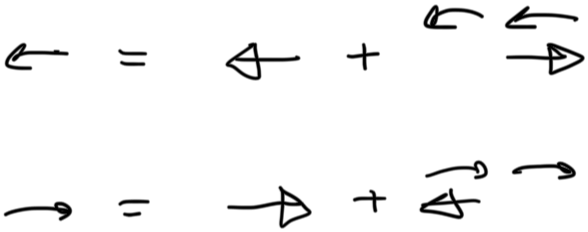
\includegraphics[width=0.3\textwidth]{src/Comet00-path-decomp1.png}
	\end{figure}

	Now, here comes the clever construction. We start from something symmetric and apply decomposition to each side respectively. The following diagram is obtained:
	\begin{figure}[H]
		\centering
		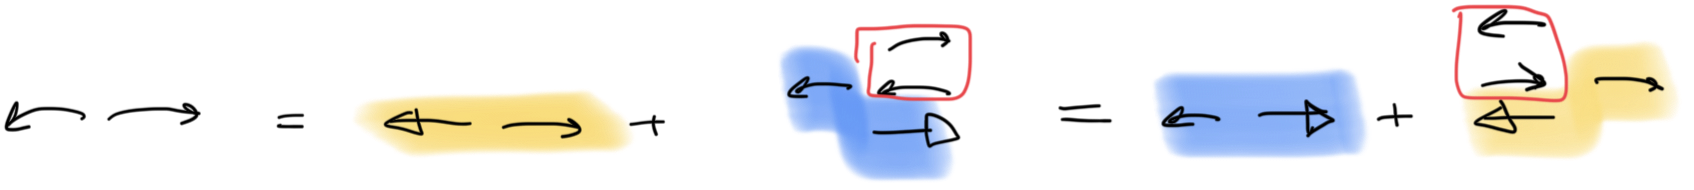
\includegraphics[width=0.8\textwidth]{src/Comet00-path-decomp2.png}
	\end{figure}

	Rearrange, and this gives:
	\begin{equation}
		\label{eqn:Comet00Fraction}
		\frac{\color{orange}(1 - \omega) \varphi(\lambda, \omega)}{\color{blue}\tilde \varphi^M(\lambda, \omega) \omega} 
		= \frac{ 1 - \tilde \varphi^{M-1}(\lambda, \theta \omega) \varphi(\lambda, \omega)}{1 - \tilde \varphi^M(\lambda, \omega)\varphi(\lambda, \theta^{-1}\omega)}
	.\end{equation} 
	Take logarithm and average in $M = 2\ldots K+1$, the R.H.S. becomes a telescoping sum. 
	\begin{align*}
	&\frac{1}{K}\sum_{M=2}^{K+1} E \log \frac{1 - \tilde \varphi^{M-1}(\lambda, \theta \omega) \varphi(\lambda, \omega)}{1 - \tilde \varphi^M(\lambda, \omega)\varphi(\lambda, \theta^{-1}\omega)}\\
	&= \frac{1}{K} \left[
	- E \log \left( 1 - \tilde \varphi^{K+1}(\lambda, \theta^{-1} \omega) \varphi(\lambda, \omega) \right) 
	+ E \log \left( 1 - \varphi(\lambda, \omega)\tilde \varphi^1(\lambda, \theta \omega) \right) 
\right] 
	.\end{align*}
	The second term is constant. Apply path decomposition again, we have
\begin{align*}
	\frac{1}{K} \left[
	- E \log \left( 1 - \tilde \varphi^{K+1}(\lambda, \theta^{-1} \omega) \varphi(\lambda, \omega) \right) \right] 
	&=  - \frac{1}{K} E \log \left( 1 - \frac{E_\omega \left[ e^{\lambda T_K; D_M} \right] }{E_\omega \left[ e^{\lambda T_K} \right] } \right)  \\
	&=  - \frac{1}{K} E \log \left( \frac{E_\omega \left[ e^{\lambda T_K; D_M^c} \right] }{E_\omega \left[ e^{\lambda T_K} \right] } \right)  
	\end{align*}
	where
	\begin{align*}
		&\frac{1}{K} E \log E_\omega \left[ e^{\lambda T_K; D_M^c} \right]\\
		&= \frac{1}{K} \sum_{j=1}^{K} E \log E_\omega \left[ e^{\lambda \tau_j}; (\tau_{-1} < \tau_j)^c \right]  \\
		&= \frac{1}{K} \sum_{j=1}^{K} E \log E_\omega \left[ e^{\lambda \tau_j}; \tau_{-j} \ge \tau_1 \right]  \\
		& \to E \log \varphi(\lambda, \omega) = \frac{1}{K} E \log E_\omega e^{\lambda T_k}
	\end{align*}
	by the Ergodic theorem. Hence, as $M \to \infty $, the fraction on the right hand side of \eqref{eqn:Comet00Fraction} vanishes. We have
	\[
		E \log \rho_0 + E \log \varphi(\lambda, \omega) - E \log \tilde\varphi^M(\lambda, \omega) = o_M(1)
	.\] 
	Take $M \to \infty $ and we obtain the claim.

	\textbf{Step 3: unconditioned LDP for backtracking.}
	Consider $\eta \in M_1^e (\Sigma)^{+, K}$. For $A \subset [1, \infty )$, we have
	\[
		P_\omega \left[ \frac{1}{n}\sum_{j=1}^{n} \tau_{-j} \in A, T_{-n, < \infty } \right] 
		= P_\omega\left[ \frac{1}{n}\sum_{j=1}^{n} \overline{\tau} _{-j}\in A \right] P_\omega \left[ T_{-n} < \infty  \right] 
	.\] 
	where
	\begin{itemize}
		\item $\lim \frac{1}{n}\log P_\omega \left[ \frac{1}{n}\sum_{j=1}^{n} \tau_{-j} \in A, T_{-n, < \infty } \right] =: - I_ \eta^{- \tau, q}(A)$ 
		\item $\frac{1}{n} \log P_\omega\left[ \frac{1}{n}\sum_{j=1}^{n} \overline{\tau} _{-j}\in A \right] \to  - I_ \eta ^{\tau, q}(A)$
		\item $\frac{1}{n} \log P_\omega \left[ T_{-n} < \infty  \right] \to E \log \rho_0$.
	\end{itemize}
	Thus
	\[
		I_ \eta^{- \tau, q}(A) = I_ \eta^{\tau, q}(A) - E \log \rho_0
	.\] 

	\textbf{Step 4: Environment Reflection.}
	Define $\eta^{\text{inv}}$ to be reflected environment. Then, $\eta \in M_1^e(\Sigma)^{-,K} \iff \eta^{\text{inv}} \in M_1^e(\Sigma)^{+,K}$. 
	
	Now, consider $\eta \in M_1^e(\Sigma)^{-,K}$. We can apply the above theorem to $\eta^{\text{inv}}$ and obtain
	\[
		I_ \eta^{\tau, q}(A) = I_ {\eta^{\text{inv}}}^{- \tau, q}(A) = I_ {\eta^{\text{inv}}}^{\tau, q}(A) - E \log \rho_0(\omega^{\text{inv}}) = _ {\eta^{\text{inv}}}^{\tau, q}(A) + E \log \rho_0
	.\]
	
\end{proof}



\subsection{Annealed LDP for hitting times.}

\begin{proof}[Proof of Theorem 5]
	\textbf{Upper bounds.}

	We begin by proving an upper bound for $\frac{1}{n} \log P\left[\frac{1}{n} \sum_{j=1}^n \tau_j \leq u\right]$, where $1<u<\infty$. We have, for $\lambda \leq 0$,

\[
P\left[\frac{1}{n} \sum_{j=1}^n \tau_j \leq u\right] \leq E\left[\exp \left(\lambda \sum_{j=1}^n \tau_j\right) \mathbf{1}_{\tau_j<\infty, j=1, \ldots, n}\right] e^{-\lambda n u}
\]


Now, this can be rewritten as expectation of log MGF w.r.t. the empirical measure:
\[
\begin{aligned}
E\left[\exp \left(\lambda \sum_{j=1}^n \tau_j\right) \mathbf{1}_{\tau_j<\infty, j=1, \ldots, n}\right] & =E\left[\prod_{j=1}^n E_\omega\left[e^{\lambda \tau_j} \mathbf{1}_{\tau_j<\infty}\right]\right] \\
& =E\left[\exp \left(\sum_{j=0}^{n-1} f\left(\lambda, \theta^j \omega\right)\right)\right] \\
& =E\left[\exp \left(n \int f(\lambda, \omega) R_n(d \omega)\right)\right]
\end{aligned}
\]

where $R_n=\frac{1}{n} \sum_{j=0}^{n-1} \delta_{\theta^j \omega} \in M_1(\Sigma)$. 

Now, by assumption, $R_n$ satisfies a L.D.P. with rate function $h(\cdot | \alpha)$. Hence, by Varadhan's Lemma , we have
\[
	\sup_{\eta \in M_1^s(\Sigma)} \left[ \int f(\lambda, \omega) \eta(d \omega) - h(\eta | \alpha) \right] 
.\] 
Note that we are taking sup in $M_1^s$, the set of stationary measures. ($R_n$ is ergodic by assumption, but linear combination of ergodic measures is in general stationary, not ergodic. In fact, any distinct ergodic measures are mutually singular, leading to infinite $h(\eta | \alpha)$, so the sup will be attained at a non-ergodic measure.)

We write the rest of the proof in a more compact form, and then we will explain the steps in detail.

\begin{align*}
	\limsup _{n \rightarrow \infty} \frac{1}{n} \log P\left[\frac{1}{n} \sum_{j=1}^n \tau_j \leq u\right]
	&\leq \inf _{\lambda \leq 0} \sup _{\eta \in M_1^s(\Sigma)}\left[\int f(\lambda, \omega) \eta(d \omega)-h(\eta \mid \alpha)-\lambda u\right] \\
	&= - \sup _{\lambda \le 0} \inf _{\eta \in M_1^s(\Sigma)} \left[ -\int f(\lambda, \omega) \eta(d \omega)+h(\eta \mid \alpha)+\lambda u \right] \\
	&\stackrel{(1)}{=} - \inf_{\eta \in M_1^s(\Sigma)} \sup_{\lambda \le 0} \left[ -\int f(\lambda, \omega) \eta(d \omega)+h(\eta \mid \alpha)+\lambda u \right] \\
	&\stackrel{(2)}{=} - \inf_{\eta \in M_1^e(\Sigma)} \sup_{\lambda \le 0} \left[ \lambda u - \int f(\lambda, \omega) \eta(d \omega)+h(\eta \mid \alpha) \right] \\
	&\stackrel{(3)}{=} - \inf_{\eta \in M_1^e(\Sigma)} \inf _{w \leq u} \left[ I_\eta^{\tau, q}(w) + h(\eta | \alpha) \right] \\
	&= - \inf _{w \leq u} I_\alpha ^{\tau, an}(w) 
.\end{align*}

\textbf{Step 1: Minimax theorem.} 
A minimax theorem in Sion \autocite[Theorem~4.2']{sionGeneralMinimax1958} can be used. See note on minimax. We just need to check the conditions: (1) the function $(\lambda, \alpha) \mapsto \lambda t-\Lambda_\alpha(\lambda)+h(\alpha \mid \eta)$ is concave in $\lambda$, (2) convex in $\alpha$, and (3) the set $\mathcal{M}_\eta$ is compact, and (4) the function is continuous.

\textbf{Step 2: Ergodic measures.}
By our assumption on the environment, we have that, for each $\overline{\eta} \in M_1^s(\Sigma)$, there exists $\eta^n \in M_1^e(\Sigma)$ such that $\eta^n \to \overline{\eta}$ both weakly and in the sense of $h(\cdot | \alpha)$. Then,
\begin{align*}
	&\inf_{\eta \in M_1^e(\Sigma)} \sup_{\lambda \le 0} \left[ \lambda u - \int f(\lambda, \omega) \eta(d \omega)+h(\eta \mid \alpha) \right]\\
	&\leq \sup_{\lambda \le 0} \left[ \lambda u - \int f(\lambda, \omega) \eta^n (d \omega)+h(\eta^n \mid \alpha) \right] \\
	&= \lambda_n u - \int f(\lambda_n, \omega) \eta^n (d \omega)+h(\eta^n \mid \alpha)\\
	&\to \lambda^* u - \int f(\lambda^*, \omega) \overline{\eta} (d \omega)+h(\overline{\eta} \mid \alpha)\\
	&= \sup_{\lambda \le 0} \left[ \lambda u - \int f(\lambda, \omega) \overline{\eta} (d \omega)+h(\overline{\eta} \mid \alpha) \right]
\end{align*}

\textbf{Step 3: Shape of the rate function.}
The final step is to show that
\[
	\sup_{\lambda \le 0} \left[ \lambda u - \int f(\lambda, \omega) \eta(d \omega)\right] = \inf_{w \leq u} I_\eta^{\tau, q}(w)
\]
By looking at the shape of the function $f(\lambda, \omega)$, we can make sense of this equality. This is because the rate function $I_\eta^{\tau, q}(\cdot)$ is convex with minimum value {\color{orange}$\int \log \rho_0(\omega) \eta(d \omega) \vee 0$} achieved at $E_\eta \tau_1$. When the walk is transient to the left, ``conditioning to hit $\infty$'' gives you the cost $\int \log \rho_0(\omega) \eta(d \omega)$ in the rate function.

The proof for upper tail is similar, though one needs to take supremum on $[0, \lambda_{\text{crit}}]$, and the modification of the argument is detailed in the erratum. \followup
This concludes the proof of the upper bound.

\textbf{Lower Bounds.}


	\[
	P_\omega \otimes \alpha(d \omega) (A) := \int_\Sigma P_\omega(A) \alpha(d \omega)
	\]

\end{proof}

